%%==================================================
%% chapter01.tex for BIT Master Thesis
%% modified by yang yating
%% version: 0.1
%% last update: Dec 25th, 2016
%%==================================================
\chapter{实验评估}
\begin{table}
    \centering
    \begin{tabular}{|>{\centering\arraybackslash}m{3cm}|>{\centering\arraybackslash}m{4cm}|>{\centering\arraybackslash}m{5cm}|}
    \hline
    FPGA & \multicolumn{2}{c|}{Zynq UltraScale + XCZU15EG-2FFVB1156 MPSoC} \\ \cline{2-3} 
     & RISC-V soft IP core & rocket-chip with N extension, 4 Core, 100MHz \\ \cline{2-3} 
     & Ethernet IP core & Xilinx AXI 1G/2.5G Ethernet Subsystem (1Gbps) \\ \hline
    Operating System & \multicolumn{2}{c|}{ReL4} \\ \hline
    Network Stack & \multicolumn{2}{c|}{smoltcp} \\ \hline
    \end{tabular}
    \caption{实验平台信息}
    \label{tab:platform_info}
    \end{table}


为了全面验证ReL4微内核系统的正确性和高效性,本章设计了一套完整的测试方案,从功能正确性、兼容性和运行效率三个维度进行评估。

在功能验证和兼容性测试方面,本文重点关注内核核心模块的功能正确性,以及对seL4的兼容性,因此采用seL4test作为功能验证和兼容性测试框架。测试结果表明,ReL4在保证基本系统调用和微内核基本功能(内存管理、任务调度、IPC等)的前提下,对seL4有着良好的兼容性。

性能评估部分采用了对比实验的方法,将ReL4与原生seL4在相同硬件平台上进行基准测试。测试指标包括特权级切换次数、IPC延迟、吞吐量等核心系统开销。实验数据显示,得益于硬件加速和异步运行时优化,ReL4在大多数测试场景中表现出更优的性能,特别是在高频IPC通信场景下,ReL4的IPC性能比seL4高出3x+。此外,通过运行真实场景下的网络服务器测试,本文验证了异步系统调用和异步IPC对微内核系统中的网络子系统有着明显收益。

下面将分别介绍功能测试与性能测试的详细细节。

\section{实验环境}
本文采用的实验平台由硬件和软件两部分组成,其详细配置参数如表\ref{tab:platform_info}所示。

在硬件平台方面,我们选用了Xilinx公司推出的Zynq UltraScale+ MPSoC系列FPGA开发板\cite{xilinx2023zynq}作为基础实验平台。该开发板搭载了基于RISC-V架构的64位四核处理器,主频配置为100MHz。值得注意的是,该处理器支持最新的N扩展指令集(RISC-V "N" Extension),为中断处理和异常控制提供了硬件级的支持。FPGA的可编程逻辑部分通过AXI总线\cite{arm2023axi}与处理器系统紧密耦合,为硬件加速器设计提供了灵活的实现空间。

软件平台采用分层架构设计,具体实现如下:
\begin{enumerate}
    \item 在SBI(Supervisor Binary Interface)层,我们移植了opensbi v1.3\cite{opensbi}作为硬件抽象层,负责处理底层硬件资源的管理和调度;
    \item 操作系统层选用ReL4微内核,该内核兼容了seL4的基本系统调用,将同步IPC从内核中移除,同时用硬件加速器对异步通知机制进行加速。
    \item 用户态运行环境集成了ReL4 Async runtime,为应用程序提供异步运行时支持;
    \item 网络子系统采用模块化设计,底层驱动使用我们开发的AXI-Net driver\cite{axima-power-axinet},该驱动通过AXI DMA引擎\cite{amd-axi-dma-controller}实现高速数据传输;
    \item 网络协议栈选用轻量级的smoltcp\cite{smoltcp-rs-smoltcp}实现,该开源协议栈经过优化后可在资源受限的嵌入式环境中高效运行。
\end{enumerate}

该实验平台的设计充分考虑了功能完备性和性能可扩展性,为后续实验验证提供了可靠的软硬件基础环境。
\section{功能测试}
ReL4的功能验证工作主要基于seL4微内核的官方测试框架seL4test\cite{sel4-sel4test}进行。作为seL4生态系统的标准测试套件,seL4test提供了全面而严格的测试用例集,涵盖系统调用、任务管理、内存管理、进程间通信(IPC)以及能力(Capability)机制等微内核核心功能模块。该测试框架采用分层测试策略,包含从基础功能验证到复杂场景测试的多层次测试用例,能够有效保证微内核实现与形式化规范的一致性。

在验证过程中,我们充分利用了ReL4与seL4的API兼容性特性。测试结果表明,ReL4能够完整通过seL4test框架中108个测试用例中的102个(具体测试结果参见表\ref{tab:seL4_test_info})。这一结果不仅验证了ReL4在核心功能实现上的正确性,同时也证实了ReL4与seL4在系统接口层面的高度兼容性。值得注意的是,如第\ref{sec:rel4_comp}节所述,由于ReL4在通知机制和IPC机制实现上的创新设计,与原生seL4存在两处关键差异,这导致部分直接调用底层系统调用和不兼容特性的测试用例需要进行适配性修改。

针对这些特殊情况,我们采取了最小化修改原则,仅对涉及差异机制的测试用例进行必要调整。具体而言,修改主要集中在以下两个方面:首先,对直接调用或间接调用\ref{sec:rel4_comp}中提到的不兼容的两个特性的测例进行少量修改,使其调用我们提供的类似的用户态库函数;其次,对IPC和通知机制的测试框架代码进行了封装改造,将运行时初始化等操作隐式包含在第一次发起IPC的操作中。这些修改严格控制在测试框架层面,并未改变测试的语义和验证目标,从而保证了测试结果的可靠性。

通过系统化的测试验证,我们确认ReL4在保持与seL4高度兼容的同时,其核心功能实现符合微内核的设计规范。测试过程中收集的详细数据(见表\ref{tab:seL4_test_info})显示,除通过IPC进行能力传递,以及多个线程接收单个Notification内核对象的不兼容场景(已经在\ref{sec:rel4_comp}中说明),ReL4能够完美支持seL4定义的其他所有核心功能特性。这一验证结果为ReL4在实际系统中的部署应用提供了坚实的功能正确性保障。


\begin{table*}[htbp]
    \centering
    \begin{tabular*}{1.0\textwidth}{@{\extracolsep{\fill}}lll}
    \toprule
    测试套			&通过情况 &说明	 \\
    \midrule
    基本系统调用			&15/15 & 非Invocation的系统调用(如Debug、Print等系统调用) \\
      通知机制			&3/4 & 除了单内核对象多接收线程之外,其余全部通过	 \\
      IPC &9/14 & 除了通过IPC进行capability传递的5个测例,其余全部通过	 \\
      错误处理  &9/9 & 主要是页错误处理测试\\
      任务管理	&11/11 & 包括线程配置和调度 \\
      能力空间管理 &10/10 & 包含Capability派生、删除、撤销等测试\\
      地址空间管理 &6/6 & 包含页表映射、物理内存映射等测试 \\
      物理内存管理 &3/3 & 包含Untyped管理与Retype接口测试  \\
      其他非单一功能测试 & 36/36 & 针对调用了上述不兼容特性的测例进行了修改,见\ref{sec:rel4_comp} \\
    \bottomrule
    \end{tabular*}
    \caption{ReL4在seL4test的测试情况} \label{tab:seL4_test_info}
  \end{table*}

\section{性能测试}
功能正确性测试虽然能够验证系统行为的合规性,但实际系统可用性还高度依赖于其运行时的性能表现。为全面评估ReL4的性能特性,本节设计了一系列精细化的性能测试实验,从不同维度考察系统的运行效率。

首先,我们采用消融实验方法评估了关键优化技术对系统性能的影响。针对用户态通知机制(U-notification)和自适应混合轮询策略,分别测试了两个因素对系统性能的影响。

在系统调用方面,我们以内存映射的系统调用为例,评估了异步系统调用对内存分配性能的提升效果。通过设计并发的内存分配压力测试,对比了传统同步调用与异步调用的性能差异。

进程间通信性能是微内核系统的关键指标。我们采用典型的Ping-Pong测试方法,测量了不同并发度、不同CPU核心数下、不同硬件资源下的平均IPC开销。

为验证系统在实际应用中的表现,我们构建了高并发TCP服务器基准测试。该测试模拟了真实网络环境中的连接建立、数据传输等典型操作。网络协议栈以进程的形式运行,服务器通过IPC请求服务,

下面将详细介绍本节的实验设计方案结实验结果。

\subsection{消融实验}
为深入评估ReL4核心优化机制的实际效果,本节设计了两组消融实验,分别针对用户态通知机制(U-notification)和自适应混合轮询策略进行定量分析。

第一个消融实验系统性地比较了U-notification与传统内核通知机制在单核与多核环境下的性能差异。如\ref{fig:ntfn_test}(a)所示,U-notification在软件实现层面通过减少页表切换和进程调度次数,显著降低了通知延迟。具体而言,在单核测试场景中,U-notification将平均延迟降低了45\%(性能提升0.8倍)。更值得注意的是,在多核测试中,传统通知机制由于依赖核间中断(IPI)唤醒接收进程,且受限于内核临界区的串行访问特性,导致接收核心必须等待发送核心完全退出内核态后才能处理中断,产生了额外的调度延迟。实验数据显示,这种设计在多核环境下造成了显著的性能退化,而U-notification通过完全在用户态完成事件通知,避免了特权级切换和进程调度开销,使得多核性能提升达到4倍。

第二个消融实验重点评估了不同事件处理策略对系统性能的影响。在固定16个客户端并发度的测试环境下,我们对比了纯中断、纯轮询以及自适应混合轮询三种模式的性能表现。如\ref{fig:ntfn_test}(b)所示,实验结果表明:纯中断模式虽然能保持较高的CPU利用率(平均>95\%),但由于中断处理固有的上下文切换开销,导致平均延迟较高(>10000 cycles);纯轮询模式虽然实现了较低的延迟(<7000 cycles),但造成了严重的CPU资源浪费(利用率<60\%)。相比之下,自适应混合轮询机制通过动态调整轮询频率和中断触发阈值,在延迟(平均8000 cycles 左右)和CPU利用率(平均92\%)之间实现了最优平衡。该机制的核心创新在于其负载感知能力,能够根据系统实际负载情况智能地切换工作模式:在低负载时倾向于轮询以降低延迟,在高负载时自动增加中断比例以提高CPU使用效率。

综合分析实验结果可以得出:U-notification通过消除内核介入带来的开销,在多核环境下展现出显著优势;而自适应混合轮询机制则通过动态策略调整,实现了延迟与资源利用率的最佳权衡。这些优化共同构成了ReL4高性能特性的技术基础,为其在实际应用场景中的优异表现提供了机制保障。

\begin{figure*}[htbp]
    \centering
    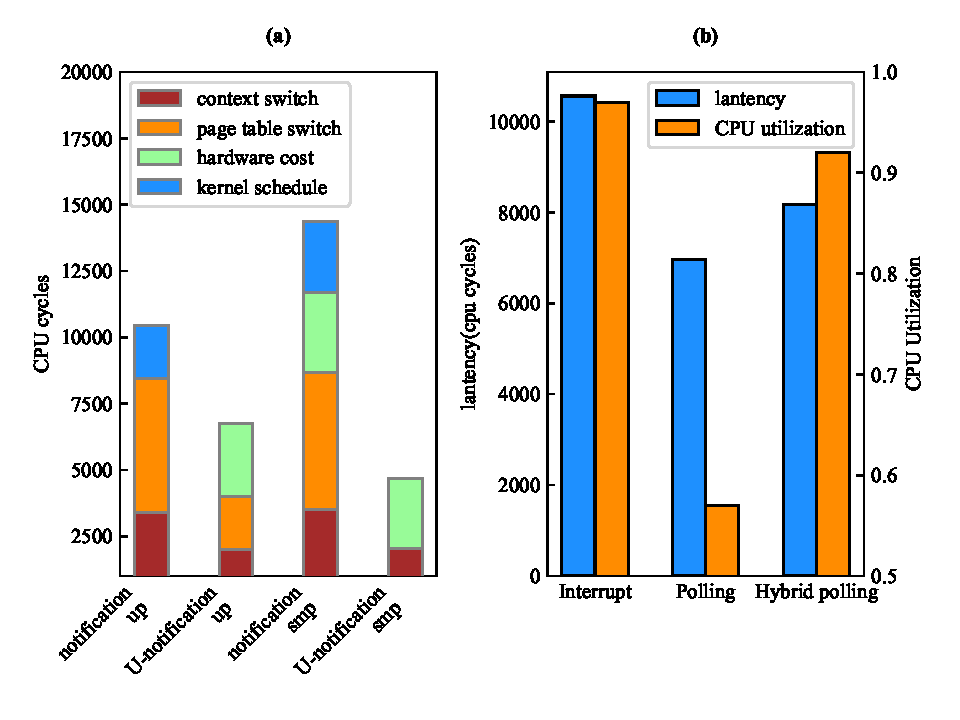
\includegraphics[width=1.0\textwidth]{figures/ntfn_test.pdf}
    \caption{U-notification与自适应混合轮询的消融实验}\label{fig:ntfn_test}
\end{figure*}

\subsection{内存分配服务器}
为深入理解异步系统调用对操作系统性能的影响,本节设计了一个基于用户态内存管理服务的对比实验。实验构建了一个典型的生产者-消费者模型,其中多个工作线程通过消息队列向核心服务线程发送内存操作请求。该设计模拟了现代系统软件中常见的内存管理场景,为评估系统调用性能提供了有说服力的测试场景。

在实验方法上,本节采用了严格的对照设计。通过保持硬件环境、工作负载等条件一致,仅改变系统调用方式(同步/异步)这一独立变量,确保了实验结果的有效性和可比性。测试过程中,我们不仅关注传统的平均CPU周期指标,还特别考察了内核交互频率这一关键参数,以全面评估不同系统调用方式对整体系统性能的影响。

实验结果如\ref{fig:syscall_test}所示,从系统调用的整体性能趋势来看,基于用户态中断的异步实现的内存分配器展现出显著的可扩展性优势。随着并发度的提高,其性能呈现近似线性的增长趋势,这一现象在并发度达到8时趋于稳定。深入分析表明,这种性能提升主要源于一个关键因素:高并发条件下批处理效应显著降低了内核陷入频率,测试数据显示在8并发时内核交互次数较同步情况减少了90\%以上,特权级切换次数的减少直接降低了上下文保存与恢复的开销,同时还增强了代码局部性。

在同步与异步实现的对比分析中,观察到一个重要的临界点现象。当并发度低于4时,同步系统调用反而展现出更好的性能表现。这一看似矛盾的现象可以通过细致的开销分解得到解释:异步机制虽然减少了特权级切换,但引入了额外的运行时管理开销(平均每个请求增加约2000个CPU周期)。量化分析显示,在并发度为2时,异步方案的总开销比同步方案高出约35\%。然而,当并发度超过4后,异步方案的优势开始显现。此时,批量处理带来的规模效应使得单次内核陷入可以处理多达4个左右请求,特权级切换的开销占比下降,从而实现了性能的反超。而基于TAIC的异步系统调用在低并发度下能够显著减少运行时的切换开销,在并发度为1的场景下,相比于用户态中断的异步系统调用,TAIC将性能提升了74\%,在单核情况下,由于需要陷入内核执行系统调用,因此相比于同步仍有所差距,而在多核情况下,基于TAIC的系统调用无需陷入内核,避免了特权级的切换,进而比同步系统调用的性能还要高出30\%,这一优势随着并发度的增加逐渐扩大到70\%。

从执行架构的角度考察,多核环境下的性能特征呈现出新的特点。当内核与客户端分布在不同的CPU核心上时,系统调用的请求处理与内核执行可以实现真正的并行化。测试数据显示,这种配置下的吞吐量比单核情况提升了约16\%。然而,值得注意的是,在用户态中断的硬件下,由于内核独占一个计算核心,其负载压力相对降低,这导致了一个意外的现象:在多核配置下,客户端陷入内核的频率反而比单核情况高出约25\%。这一现象揭示了内核负载与客户端行为之间复杂的相互作用关系,为后续的系统优化提供了新的研究方向。

\begin{figure*}[htbp]
    \centering
    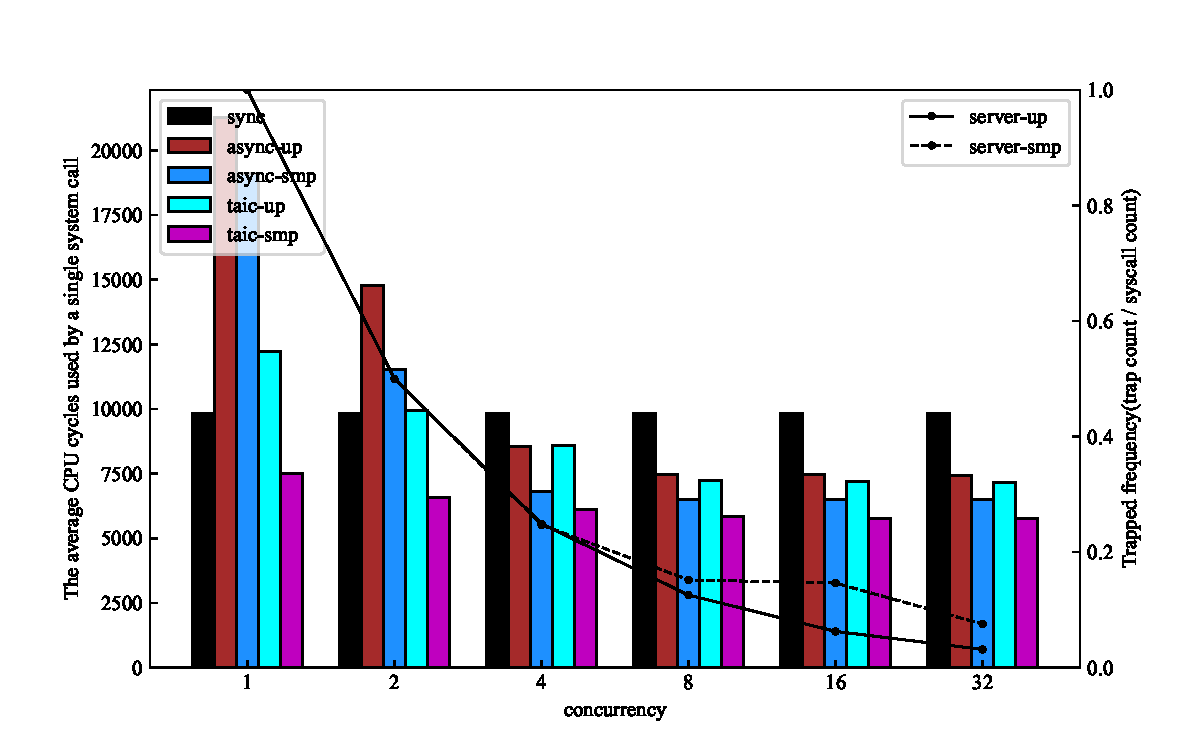
\includegraphics[width=1.0\textwidth]{figures/syscall_test.pdf}
    \caption{内存分配服务器性能测试实验}\label{fig:syscall_test}
\end{figure*}

\subsection{同步IPC vs. 异步IPC}
为深入理解异步IPC的性能特性,本节设计了一套乒乓测试方案,通过控制服务端与客户端进程的交互模式,排除了其他系统组件的干扰,专门考察同步与异步IPC的路径差异。如\ref{fig:ipc_test}所示,实验结果揭示了若干重要的性能特征。

同步IPC的性能表现呈现出明显的场景依赖性。在多核环境下,由于fast-path检查必然失败,所有IPC请求都需要通过核间中断进行传递,导致性能显著下降。测试数据显示,多核同步IPC的延迟比单核情况增加了近3倍。而在单核场景下,当满足fast-path条件时(即线程优先级匹配且消息长度短),同步IPC可以绕过复杂的消息解码和调度流程,性能提升幅度达到167\%。然而,实际应用中的统计表明,由于严格的检查条件限制,fast-path优化的适用场景相当有限,仅在单核且C/S请求模式下的短消息传递才能生效。

异步IPC则展现出截然不同的性能特征。随着并发量的增加,其性能呈现明显的改善趋势。这一现象可以从两个层面进行解释:首先,自适应U-notification机制会根据负载情况动态调整通知频率,在高并发时减少不必要的中断;其次,批量处理效应使得固定开销得以分摊。值得注意的是,多核环境下的性能优势呈现出有趣的动态变化:在低并发时(1-4个并发请求),多核配置比单核快52\%,这得益于真正的并行处理;但随着并发度增加(超过16个请求),优势逐渐缩小至17\%。深入分析表明,这是由于专用服务端核心的负载不足,导致中断频率过高,反而限制了整体吞吐量。

同步与异步IPC的性能对比揭示了一个关键的系统设计权衡。在低并发场景(并发度=1)下,异步IPC由于额外的用户态中断(2次)和调度器开销,其性能比无fast-path的同步IPC低31\%,比带fast-path的同步IPC更低达249\%。然而,随着并发度增加,异步IPC的优势快速显现:当并发度达到8时,其性能已超过带fast-path的同步IPC;在32并发时,性能优势达到76\%。这种动态特性说明,异步IPC特别适合现代高并发应用场景,而同步IPC则在特定低并发场景下可能更具优势。

而对比TAIC加速之后的异步IPC,我们可以明显看到在低并发场景(并发度=1)下,异步IPC性能提高了84\%,不仅超越了普通同步IPC,而且接近fast-path优化版本。这一提升主要源于TAIC的两个关键创新:首先,硬件自动化处理中断信号消除了软件中断处理的开销,改善了程序局部性并减少了上下文保存开销;其次,硬件自动唤醒协程避免了避免了运行时调度器的频繁操作。随着并发度提高,虽然中断优化的收益被均摊,但TAIC的唤醒机制优化仍能带来48\%的性能提升,这主要得益于其减少了运行时调度开销。

综合测试结果表明,异步IPC在多核环境下始终展现出良好的性能表现。TAIC加速技术进一步拓展了其优势范围,使其在低并发场景也具备竞争力。虽然在单核低并发场景下异步IPC存在一定劣势,但随着并发度的增加,其性能优势迅速显现,在当今普遍的多核高并发计算环境下,结合TAIC等硬件加速技术的异步IPC架构具有显著的应用价值。


\begin{figure*}[htbp]
    \centering
    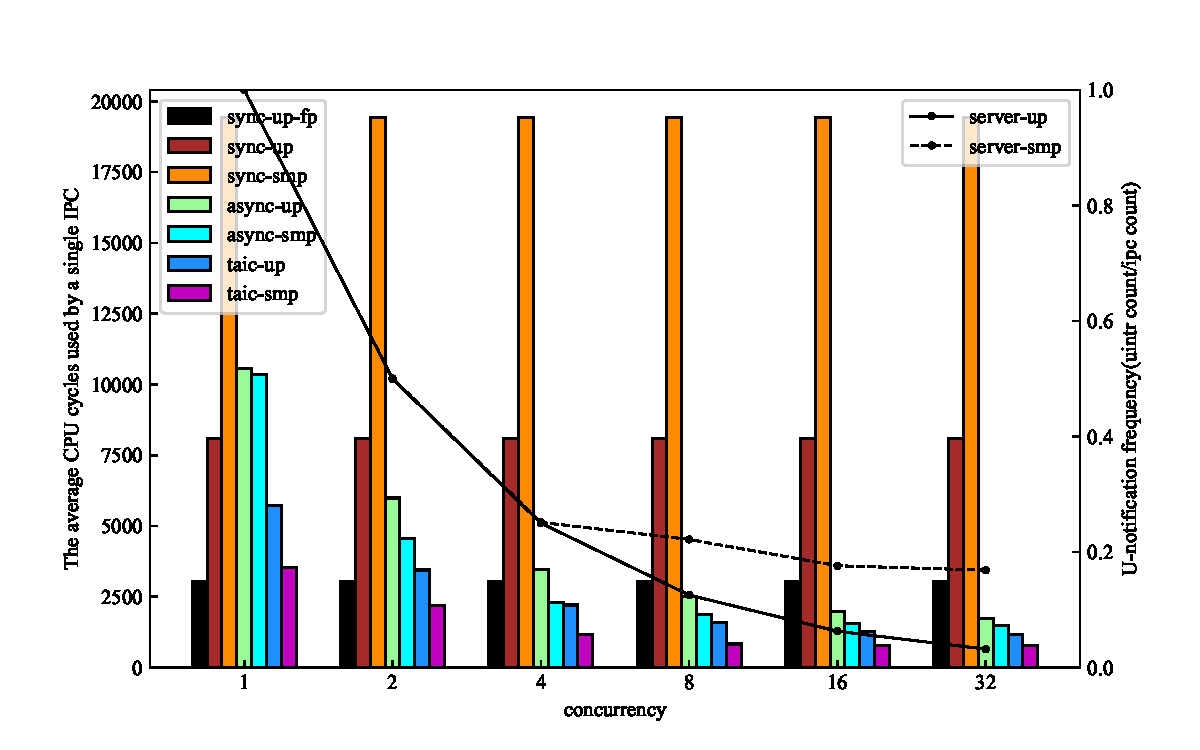
\includegraphics[width=1.0\textwidth]{figures/ipc_test.pdf}
    \caption{IPC对比测试实验}\label{fig:ipc_test}
\end{figure*}

\subsection{TCP 服务器}

为验证异步IPC在实际应用中的性能优势,本节设计并实现了一个完整的TCP服务器基准测试系统。该测试架构采用微内核中典型的模块化设计,充分模拟了真实网络应用场景中的数据处理流程。

如\ref{fig:tcp_test}所示,测试系统的客户端部署在标准PC上,通过以太网与运行在FPGA开发板上的ReL4系统建立网络连接。客户端采用多线程架构,每个线程维护独立的TCP连接,持续发送64字节的小数据包并等待服务器响应,统计响应延迟和吞吐量,用于评估系统在高并发小包处理场景下的性能表现。

\begin{figure*}[htbp]
    \centering
    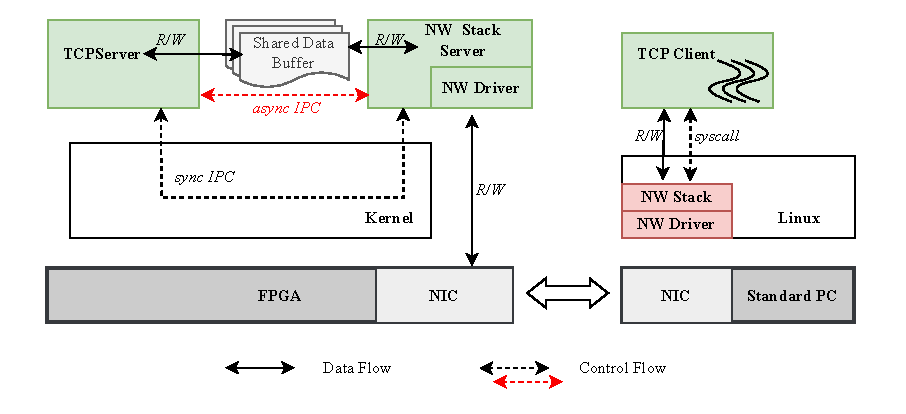
\includegraphics[width=1.0\textwidth]{figures/tcp_test_framework.drawio.pdf}
    \caption{TCP测试场景示意图}\label{fig:tcp_test}
\end{figure*}

在ReL4系统内部,网络处理流程采用模块化设计。网络协议栈服务器(NW Stack Server)作为核心数据平面组件,直接与网卡驱动交互,负责底层数据包的收发和协议处理。该服务器集成了开源的smoltcp协议栈实现,能够高效维护大量连接状态信息。通过精心设计的共享缓冲区机制,NW Stack Server与上层TCP Server之间实现了零拷贝数据传输,最大限度地减少了内存复制开销。

TCP Server作为应用层服务,通过IPC机制与NW Stack Server进行通信。这种架构设计使得网络协议处理和业务逻辑处理能够并行执行,充分发挥多核处理器的计算能力。性能指标采集方面,客户端会精确测量每个请求的端到端延迟,并统计单位时间内的消息吞吐量,为系统评估提供全面的性能数据。

需要注意的是,由于同步IPC在架构上存在固有局限,无法支持连接的多路复用,因此在同步配置下,每个TCP连接都需要独立的服务线程进行处理。这种设计虽然保证了功能正确性,但导致了显著的资源开销和性能下降。相比之下,异步IPC架构能够实现真正的连接多路复用,单个服务线程即可高效处理大量并发连接,展现出明显的性能优势。

\begin{figure*}[htbp]
    \centering
    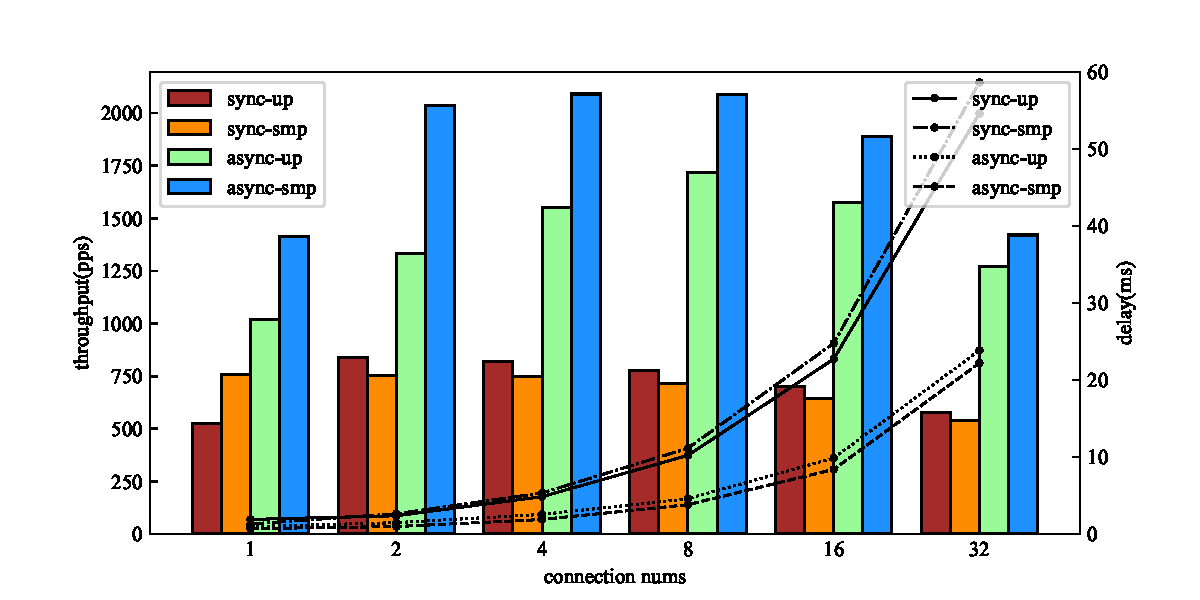
\includegraphics[width=1.0\textwidth]{figures/tcp_test.pdf}
    \caption{TCP服务器性能测试实验}\label{fig:tcp_test_res}
\end{figure*}

如\ref{fig:tcp_test_res}所示,系统吞吐量与延迟随并发度的变化呈现出典型的非线性关系。在初始阶段(1-8个并发连接),吞吐量随并发度增加而增长,这反映了系统资源尚未达到饱和状态。当并发度超过临界值(约8个连接)后,系统进入过载状态,吞吐量开始下降。这一现象可以通过中断处理模型来解释:随着并发连接数增加,网卡中断频率呈线性上升,导致CPU将大量时间消耗在中断上下文切换上。同时,共享资源(如协议栈缓冲区)的竞争加剧,进一步降低了系统效率。与吞吐量的抛物线特征不同,端到端延迟在整个测试范围内保持单调递增,这符合排队论的基本原理,即系统负载增加必然导致请求等待时间延长。

同步与异步架构的性能对比展示了微内核异步IPC的设计优势。即使在低并发场景(1-4个连接)下,异步IPC架构已展现出显著优势,其吞吐量比同步实现高出85-120\%,平均延迟降低约40\%。这种优势源于异步架构的两个关键特性:首先,它避免了频繁的内核态切换,使得网络中断能够被及时响应;其次,其事件驱动模型消除了传统多线程架构中的上下文切换开销。随着并发度增加,同步实现的多线程架构暴露出严重的扩展性问题。在4个连接时,性能差距达到峰值(192\%)。值得注意的是,即使在最大测试负载下,异步架构仍保持120\%的性能优势,证明了其在高压环境下的稳定性。

多核扩展性分析揭示了更深层次的架构差异。异步IPC实现能够有效利用多核资源,在双核配置下最好情况能实现接52\%的加速比,同时将平均延迟降低约52\%。这种良好的扩展性得益于异步IPC几乎无需内核参与,避免了内核锁的竞争,实现了最大化并行。相比之下,同步IPC在多核环境中的表现反常地劣于单核情况(性能下降约7\%)。通过性能剖析发现,这种退化主要来自两个方面:核间中断引入的额外开销,以及核间中断导致陷入内核而产生的TLB shootdown性能惩罚。特别是在小数据包处理场景下,同步实现的核心局部性显著恶化,进一步放大了多核环境下的性能劣势。

上面的测试结果表明:异步IPC在实际应用场景中有利于多路复用的实现,可以有效减少特权级切换的开销,同时提升系统的多核扩展性,进而提升系统的整体性能。

\section{本章小结}
本章通过系统的实验评估,从功能正确性、兼容性和运行效率三个维度对ReL4微内核系统进行了全面验证。实验结果表明,ReL4在保持与seL4高度兼容的同时,通过创新的异步架构设计和硬件加速机制,显著提升了微内核系统的整体性能。

在功能验证方面,基于seL4test标准测试框架的实验数据表明,ReL4能够完整支持微内核的核心功能模块,包括任务管理、内存管理和能力机制等。特别值得注意的是,除与异步架构设计直接相关的少数测试项外,系统展现出与seL4良好的兼容性,这为现有seL4生态向ReL4的平滑迁移提供了重要保障。

性能评估部分通过多组对照实验揭示了ReL4架构的性能优势。消融实验结果表明,用户态通知机制(U-notification)相比传统内核通知方式,在多核环境下可降低45\%的延迟;而自适应混合轮询策略则实现了延迟与CPU利用率的最佳平衡。系统调用性能测试显示,异步机制在高并发场景(>32并发度)下展现出显著的批处理效应,使内核交互频率降低90\%以上。IPC性能对比实验进一步证实,异步IPC相比于同步IPC,在高并发场景下有着显著优势,TAIC硬件加速技术使异步IPC在低并发场景下的性能提升达84\%,接近同步IPC的性能,同时保持了在高并发场景下的优势。

实际应用场景的测试结果更具说服力。TCP服务器基准测试表明,即使在低并发条件下,异步架构的吞吐量仍比同步实现高出85-120\%,且随着并发度增加,性能优势持续扩大。多核环境下的测试数据尤其值得关注:异步架构在双核配置下实现了接近线性的加速比,而同步实现反而因核间通信开销出现性能退化,这一对比充分证明了异步架构在多核环境下的扩展性优势。

综合实验数据可以得出,ReL4通过体系结构创新,在保证功能正确性的前提下,有效解决了传统微内核系统在性能方面的固有瓶颈。异步IPC架构与硬件加速技术的结合,使系统在保持微内核安全特性的同时,获得了接近宏内核的性能表现,为高安全需求场景下的系统设计提供了新的技术路径。